\RequirePackage{amsthm} %https://tex.stackexchange.com/questions/687324/unknown-theoremstyle-warning-with-springer-nature-template
\documentclass[sn-mathphys-num,iicol]{sn-jnl}

%\usepackage{sn-jnl.sty}
\usepackage{graphicx}%
\usepackage{multirow}%
\usepackage{amsmath,amssymb,amsfonts}%
\usepackage{amsthm}%
\usepackage{physics}
\usepackage{siunitx}
\usepackage{mathrsfs}%
\usepackage[title]{appendix}%
\usepackage{xcolor}%
\usepackage{textcomp}%
\usepackage{manyfoot}%
\usepackage{booktabs}%
\usepackage{algorithm}%
\usepackage{algorithmicx}%
\usepackage{algpseudocode}%
\usepackage{listings}%
\usepackage{newtxmath}%
\usepackage[tiny]{titlesec}%
\usepackage[ngerman]{babel}

\theoremstyle{thmstyleone}
\newtheorem{theorem}{Theorem}
\newtheorem{proposition}[theorem]{Proposition}

\theoremstyle{thmstyletwo}
\newtheorem{remark}{Remark}

\theoremstyle{thmstylethree}
\newtheorem{definition}{Definition}

\raggedbottom

\newcommand{\td}{\text{d}}

\titleformat{\subsection}{}{\thesubsection}{1em}{\itshape}

\begin{document}
        
\title{Praktikum 4 -- Versuch 402: Quantelung von Energie}
\author*[1]{\fnm{Jonas} \sur{Wortmann}}\email{s02jwort@uni-bonn.de}
\author*[1]{\fnm{Angelo} \sur{Brade}}\email{s72abrad@uni-bonn.de}
\affil*[1]{Rheinische Friedrich--Wilhelms--Universität, Bonn}

\maketitle

\newpage
\section{Einleitung}
Elektronen emittieren bzw.\ absorbieren beim Übergang zwischen Orbitalen Photonen mit einer diskreten Energie.
Diese Energie ist gequantelt in Vielfache des \textsc{Planck}'schen Wirkungsquantums $h$.
Um die Größe der Quantelung zu bestimmen wird der Photoeffekt und die Messung der \textsc{Balmer}--Serie von Hg verwendet.

\section{Photoelektrische Bestimmung von $h$.}
\subsection{Experimenteller Aufbau}
Der experimentelle Aufbau ist in Abb.\ (\ref{fig:aufbau_photoeffekt}) zu sehen.
Die Hg--Lampe diente als Lichtquelle.
Mit der Blende und der Linse wurde die Intensität und Breite des Lichtstrahls so eingestellt, dass ein fokussierter Punkt auf der Photokathode zu sehen war.
Dabei wurde darauf geachtet, dass der Lichtstrahl nicht die Anode berührte.
Zur Vermeidung von Streulicht wurde über die Kathode--Anode--Anordnung eine Blende gestülpt, mit einem Rohrausschnitt, welcher auf das Filterrad zeigte.
Mit Hilfe des Filterrades wählte man verschiedene Wellenlängen zur Beobachtung aus.

Das Gegenfeld konnte mit einer separaten Spannung eingestellt und variiert werden.
Da die Spannnug, die für das Gegenfeld zur Verfügung stand, bis zu $\SI{12}{V}$ ausgeben kann, wurde diese mit einem Spannungsteiler auf $U'=\tfrac{R_1}{R_1+R_2}U=\tfrac{\SI{100}{\ohm}}{\SI{100}{\ohm}+\SI{333}{\ohm}}12V=\SI{2.77}{V}$ gedrosselt.
\begin{figure}[h]
        \centering
        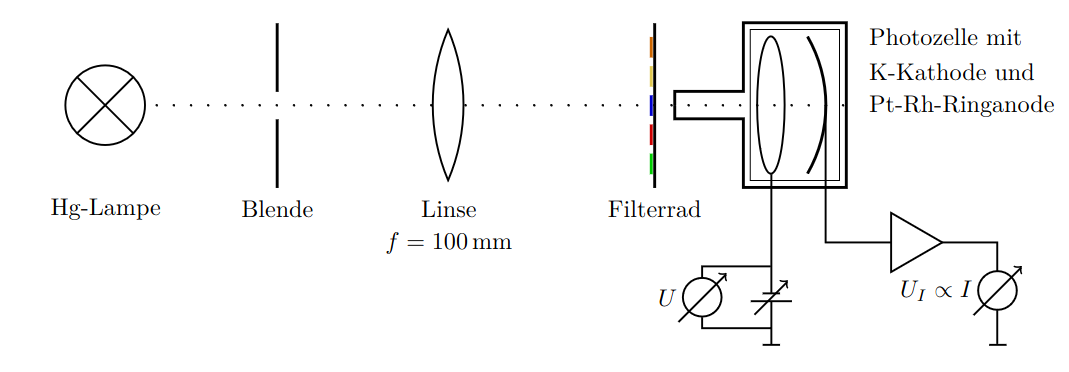
\includegraphics[width=.5\textwidth]{402_aufbau_photoeffekt.png}
        \caption{Experimenteller Aufbau zum Photoeffekt.} \label{fig:aufbau_photoeffekt}
\end{figure}

\subsection{Theoretischer Hintergrund}
Das \textsc{Fermi}--Niveau beschreibt das höchste noch besetzte Energieniveau in einem Atom, welches aufgrund des \textsc{Pauli}--Prinzips noch besetzt werden darf.
Die Austrittsarbeit ist die Arbeit die benötigt wird, um ein Elektron aus diesem Energieniveau zu heben und vom dem Atoms zu lösen.
Für verschiedene Atome ist dieses Level, wegen ihrer unterschiedlichen Elektronanzahl, nicht gleich.
Makroskopisch zeigt sich dies in unterschiedlichen Austrittsarbeiten für verschiedene Materialien, wie z.B.\ für die Anode und die Kathode im experimentellen Aufbau.

Solche Energieniveaus können mit dem Bänderschema verdeutlicht werden.
Eine mögliche Anordnung ist in Abb.\ (\ref{fig:bänderschema}) gezeigt.
Die gestrichelten Linien unten mit den schrägen Linien darunter geben die jeweiligen \textsc{Fermi}--Niveaus an.
$W_\text{K}$ und $W_\text{A}$ geben die Austrittsarbeit an.
Die alleinstehende gestrichelte Linie ist das Vakuumniveau.

Werden Anode und Kathode miteinander verbunden, so gleichen sich ihre \textsc{Fermi}--Niveaus aus und es entsteht eine Potentialdifferenz von $U_\text{KA}$ zum Vakuumsniveau zwischen Anode und Kathode.
Wird eine Spannung zwischen Anode und Kathode aufgebaut, so verschieben sich die \textsc{Fermi}--Niveaus und es baut sich eine weitere Potentialdifferenz $U_\text{G}$ auf.

Trifft ein Photon auf die Kathode, so lässt sich folgende Gleichung zwischen der Energie des Photons und der Energie des Elektrons aufstellen, mit $eU_0$ der kinetischen Energie der Elektronen
\begin{align} 
        \Leftrightarrow && E_\gamma =h\nu &=eU_0-eU_\text{KA}+W_\text{K}=E_{e^-}&&\\
        \Leftrightarrow &&&=eU_0-\left(W_\text{K}-W_\text{A}\right)+W_\text{K}&&\\
        \Leftrightarrow &&&=eU_0+W_\text{A}&&
.\end{align} 
\begin{figure}[h]
        \centering
        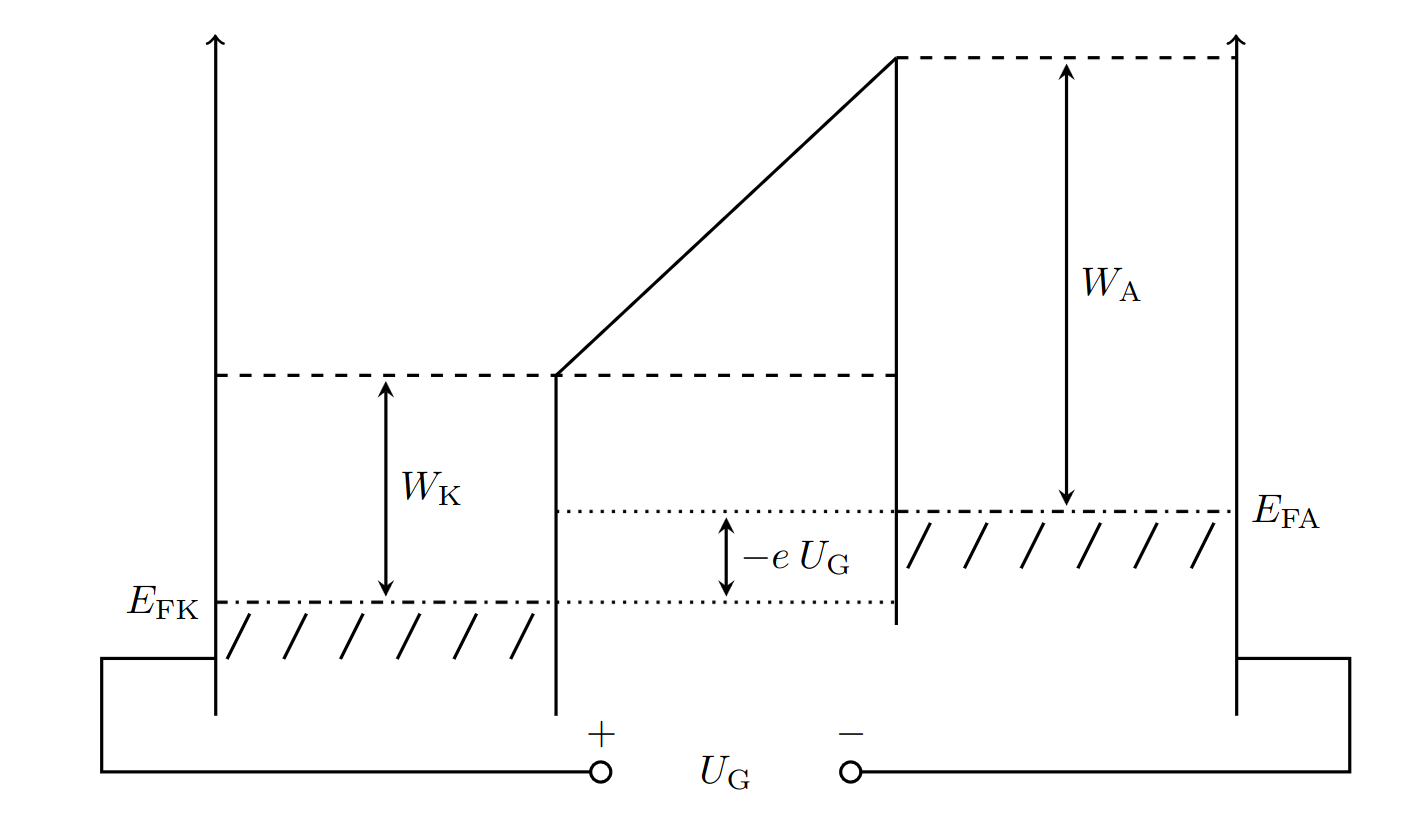
\includegraphics[width=.5\textwidth]{402_austrittsarbeit.png}
        \caption{Bänderschema der Anode und Kathode bei anlegen einer äußeren Spannung.\cite{Anleitung402}} \label{fig:bänderschema}
\end{figure}

\subsection{Durchführung \& Auswertung}
Die Messung des Photostroms und des Gegenfeldes erfolgte über zwei DMMs.
Jede Messung wurde zwei mal durchgeführt und jeweils der Mittelwert verwendet, da die Intensität der Hg--Lampe schwankt.

Die Spannung des Gegenfeldes wurde für alle Interferenzfilter ($\SI{305}{nm}$, $\SI{365}{n m}$, $\SI{436}{n m}$, $\SI{546}{n m}$ und $\SI{578}{n m}$) von der maximalen Spannung ($\approx \SI{2.77}{V}$) bis zur minimalen Spannung $(\approx \SI{0.0006}{V}$) variiert und der Photostrom gemessen.
Der Anodenstrom $I_0$, der von der Anode zu Kathode fließt, wenn die Gegenspannung maximal ist, wurde jeweils gesondert gemessen, um diesen in der Auswertung von der Messung zu subtrahieren.

Bis zu einer gewissen Gegenfeldspannung $U_\text{G}=U_0$ fließt kein Photostrom $I$; ab $U_0$ fließt dieser mit einem quadratischen Zusammenhang zu $U_G$.

Für die Auswertung wird $\,\sqrt[]{I-I_0}$ -- der Photostrom $I$ abzüglich $I_0$ unter der Wurzel -- gegen die Gegenfeldspannung $U_G$ aufgetragen.
Die Graphen finden sich im Appendix von Abb.\ (\ref{fig:photo_auswertung_305}) bis Abb.\ (\ref{fig:photo_auswertung_578}).

Ein Geradenfit wird für alle Messdaten, die im quadratischen Bereich liegen durchgeführt.
Die Messpunkte, die kein quadratisches Verhalten zeigen, geben des Strom von der Anode zur Kathode an und werden nicht berücksichtigt.
$\chi ^2/\text{ddof}$ ist für alle Geraden viel kleiner als der ideale Wert 1.
Diese Diskrepanz ist hier nicht zu kleiner Fehler sondern einer Überfittung der Geraden zuzuordnen.
Die Nullstelle der Fitgeraden liefert genau den Wert der Gegenspannung, bei der kein Photostrom fließt.

\begin{table}[h]
        \begin{tabular}{cc}
                $\lambda $ & $U_0$ \\
                \hline
                $\SI{305}{n m}$ & $\SI{-1.1806+-0.0093}{V}$ \\
                $\SI{365}{n m}$ & $\SI{-1.509+-0.017}{V}$ \\
                $\SI{436}{n m}$ & $\SI{-0.951+-0.011}{V}$ \\
                $\SI{546}{n m}$ & $\SI{-0.2615+-0.0057}{V}$ \\
                $\SI{578}{n m}$ & $\SI{-0.388+-0.015}{V}$ 
        \end{tabular}
\end{table}
Trägt man diese Werte gegen die jeweilige Frequenz des Lichts auf, so lässt sich ein Geradenfit durchführen, dessen Steigung genau gleich dem \textsc{Planck}'schen Wirkungsquantum ist.
Dieser Plot ist in Abb.\ (\ref{fig:austrittsarbeit}) zu sehen.
$\chi ^2/\text{ddof}$ ist viel größer als 1, weil sich die Fehler, durch die kleinen Messfehler, in der Fehlerfortpflanzung minimiert haben.
\begin{figure*}[t]
        \centering
        % GNUPLOT: LaTeX picture with Postscript
\begingroup
  \makeatletter
  \providecommand\color[2][]{%
    \GenericError{(gnuplot) \space\space\space\@spaces}{%
      Package color not loaded in conjunction with
      terminal option `colourtext'%
    }{See the gnuplot documentation for explanation.%
    }{Either use 'blacktext' in gnuplot or load the package
      color.sty in LaTeX.}%
    \renewcommand\color[2][]{}%
  }%
  \providecommand\includegraphics[2][]{%
    \GenericError{(gnuplot) \space\space\space\@spaces}{%
      Package graphicx or graphics not loaded%
    }{See the gnuplot documentation for explanation.%
    }{The gnuplot epslatex terminal needs graphicx.sty or graphics.sty.}%
    \renewcommand\includegraphics[2][]{}%
  }%
  \providecommand\rotatebox[2]{#2}%
  \@ifundefined{ifGPcolor}{%
    \newif\ifGPcolor
    \GPcolortrue
  }{}%
  \@ifundefined{ifGPblacktext}{%
    \newif\ifGPblacktext
    \GPblacktexttrue
  }{}%
  % define a \g@addto@macro without @ in the name:
  \let\gplgaddtomacro\g@addto@macro
  % define empty templates for all commands taking text:
  \gdef\gplbacktext{}%
  \gdef\gplfronttext{}%
  \makeatother
  \ifGPblacktext
    % no textcolor at all
    \def\colorrgb#1{}%
    \def\colorgray#1{}%
  \else
    % gray or color?
    \ifGPcolor
      \def\colorrgb#1{\color[rgb]{#1}}%
      \def\colorgray#1{\color[gray]{#1}}%
      \expandafter\def\csname LTw\endcsname{\color{white}}%
      \expandafter\def\csname LTb\endcsname{\color{black}}%
      \expandafter\def\csname LTa\endcsname{\color{black}}%
      \expandafter\def\csname LT0\endcsname{\color[rgb]{1,0,0}}%
      \expandafter\def\csname LT1\endcsname{\color[rgb]{0,1,0}}%
      \expandafter\def\csname LT2\endcsname{\color[rgb]{0,0,1}}%
      \expandafter\def\csname LT3\endcsname{\color[rgb]{1,0,1}}%
      \expandafter\def\csname LT4\endcsname{\color[rgb]{0,1,1}}%
      \expandafter\def\csname LT5\endcsname{\color[rgb]{1,1,0}}%
      \expandafter\def\csname LT6\endcsname{\color[rgb]{0,0,0}}%
      \expandafter\def\csname LT7\endcsname{\color[rgb]{1,0.3,0}}%
      \expandafter\def\csname LT8\endcsname{\color[rgb]{0.5,0.5,0.5}}%
    \else
      % gray
      \def\colorrgb#1{\color{black}}%
      \def\colorgray#1{\color[gray]{#1}}%
      \expandafter\def\csname LTw\endcsname{\color{white}}%
      \expandafter\def\csname LTb\endcsname{\color{black}}%
      \expandafter\def\csname LTa\endcsname{\color{black}}%
      \expandafter\def\csname LT0\endcsname{\color{black}}%
      \expandafter\def\csname LT1\endcsname{\color{black}}%
      \expandafter\def\csname LT2\endcsname{\color{black}}%
      \expandafter\def\csname LT3\endcsname{\color{black}}%
      \expandafter\def\csname LT4\endcsname{\color{black}}%
      \expandafter\def\csname LT5\endcsname{\color{black}}%
      \expandafter\def\csname LT6\endcsname{\color{black}}%
      \expandafter\def\csname LT7\endcsname{\color{black}}%
      \expandafter\def\csname LT8\endcsname{\color{black}}%
    \fi
  \fi
    \setlength{\unitlength}{0.0500bp}%
    \ifx\gptboxheight\undefined%
      \newlength{\gptboxheight}%
      \newlength{\gptboxwidth}%
      \newsavebox{\gptboxtext}%
    \fi%
    \setlength{\fboxrule}{0.5pt}%
    \setlength{\fboxsep}{1pt}%
    \definecolor{tbcol}{rgb}{1,1,1}%
\begin{picture}(7200.00,4320.00)%
    \gplgaddtomacro\gplbacktext{%
      \csname LTb\endcsname%%
      \put(634,619){\makebox(0,0)[r]{\strut{}$0.2$}}%
      \csname LTb\endcsname%%
      \put(634,1062){\makebox(0,0)[r]{\strut{}$0.4$}}%
      \csname LTb\endcsname%%
      \put(634,1505){\makebox(0,0)[r]{\strut{}$0.6$}}%
      \csname LTb\endcsname%%
      \put(634,1947){\makebox(0,0)[r]{\strut{}$0.8$}}%
      \csname LTb\endcsname%%
      \put(634,2390){\makebox(0,0)[r]{\strut{}$1$}}%
      \csname LTb\endcsname%%
      \put(634,2833){\makebox(0,0)[r]{\strut{}$1.2$}}%
      \csname LTb\endcsname%%
      \put(634,3276){\makebox(0,0)[r]{\strut{}$1.4$}}%
      \csname LTb\endcsname%%
      \put(634,3719){\makebox(0,0)[r]{\strut{}$1.6$}}%
      \csname LTb\endcsname%%
      \put(731,425){\makebox(0,0){\strut{}$5$}}%
      \csname LTb\endcsname%%
      \put(1347,425){\makebox(0,0){\strut{}$5.5$}}%
      \csname LTb\endcsname%%
      \put(1962,425){\makebox(0,0){\strut{}$6$}}%
      \csname LTb\endcsname%%
      \put(2578,425){\makebox(0,0){\strut{}$6.5$}}%
      \csname LTb\endcsname%%
      \put(3193,425){\makebox(0,0){\strut{}$7$}}%
      \csname LTb\endcsname%%
      \put(3809,425){\makebox(0,0){\strut{}$7.5$}}%
      \csname LTb\endcsname%%
      \put(4424,425){\makebox(0,0){\strut{}$8$}}%
      \csname LTb\endcsname%%
      \put(5039,425){\makebox(0,0){\strut{}$8.5$}}%
      \csname LTb\endcsname%%
      \put(5655,425){\makebox(0,0){\strut{}$9$}}%
      \csname LTb\endcsname%%
      \put(6270,425){\makebox(0,0){\strut{}$9.5$}}%
      \csname LTb\endcsname%%
      \put(6886,425){\makebox(0,0){\strut{}$10$}}%
    }%
    \gplgaddtomacro\gplfronttext{%
      \csname LTb\endcsname%%
      \put(170,2169){\rotatebox{-270}{\makebox(0,0){\strut{}$U_0/\SI{}{V}$}}}%
      \csname LTb\endcsname%%
      \put(3809,135){\makebox(0,0){\strut{}$\nu / \SI{}{10^{14} Hz}$}}%
      \csname LTb\endcsname%%
      \put(6123,1083){\makebox(0,0)[r]{\strut{}$U_0$ Datenpunkte}}%
      \csname LTb\endcsname%%
      \put(6123,890){\makebox(0,0)[r]{\strut{}$f(\nu)=\SI{0.228 +- 0.065}{V/\ 10^{14} Hz}\cdot \nu \SI{-0.90 +- 0.45}{V}$}}%
      \csname LTb\endcsname%%
      \put(3809,4009){\makebox(0,0){\strut{}$W_A=\SI{-0.90 +- 0.45}{eV}$, $\text{h}=\SI{0.0228 +- 0.0065 }{eVs} \cdot 10^{-15} $ und $\chi^2/\text{ddof}=752.338$}}%
    }%
    \gplbacktext
    \put(0,0){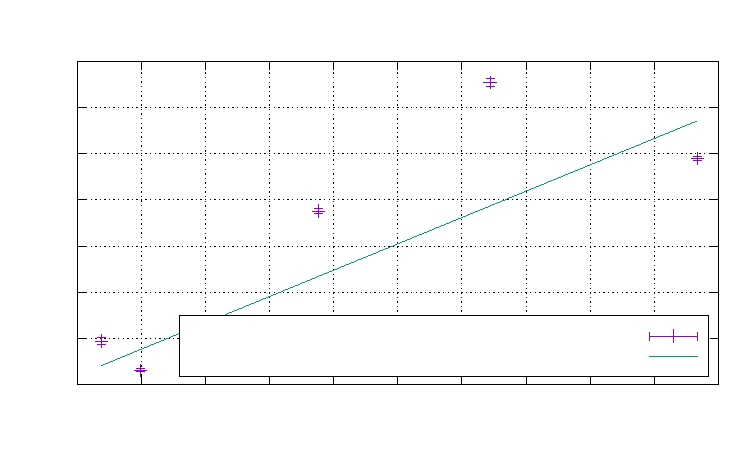
\includegraphics[width={360.00bp},height={216.00bp}]{Austritsarbeit}}%
    \gplfronttext
  \end{picture}%
\endgroup

        \caption{a} \label{fig:austrittsarbeit}
\end{figure*}
Es ergibt sich ein Wert von
\begin{align} 
        h=\SI{0.0228+-0.002e-15}{eVs}
.\end{align} 
Der aktuelle CODATA Wert (letzer Zugriff: 2024-11-23) ist
\begin{align} 
        h'\approx \SI{4.136e-15}{eVs}
.\end{align} 
Die Abweichung des gemessenen Werts liegt daher bei ca.\ $100\%$.

\section{\textsc{Balmer}--Serie}

\clearpage
\section{Appendix}
\begin{figure*}[h]
        \centering
        % GNUPLOT: LaTeX picture with Postscript
\begingroup
  \makeatletter
  \providecommand\color[2][]{%
    \GenericError{(gnuplot) \space\space\space\@spaces}{%
      Package color not loaded in conjunction with
      terminal option `colourtext'%
    }{See the gnuplot documentation for explanation.%
    }{Either use 'blacktext' in gnuplot or load the package
      color.sty in LaTeX.}%
    \renewcommand\color[2][]{}%
  }%
  \providecommand\includegraphics[2][]{%
    \GenericError{(gnuplot) \space\space\space\@spaces}{%
      Package graphicx or graphics not loaded%
    }{See the gnuplot documentation for explanation.%
    }{The gnuplot epslatex terminal needs graphicx.sty or graphics.sty.}%
    \renewcommand\includegraphics[2][]{}%
  }%
  \providecommand\rotatebox[2]{#2}%
  \@ifundefined{ifGPcolor}{%
    \newif\ifGPcolor
    \GPcolortrue
  }{}%
  \@ifundefined{ifGPblacktext}{%
    \newif\ifGPblacktext
    \GPblacktexttrue
  }{}%
  % define a \g@addto@macro without @ in the name:
  \let\gplgaddtomacro\g@addto@macro
  % define empty templates for all commands taking text:
  \gdef\gplbacktext{}%
  \gdef\gplfronttext{}%
  \makeatother
  \ifGPblacktext
    % no textcolor at all
    \def\colorrgb#1{}%
    \def\colorgray#1{}%
  \else
    % gray or color?
    \ifGPcolor
      \def\colorrgb#1{\color[rgb]{#1}}%
      \def\colorgray#1{\color[gray]{#1}}%
      \expandafter\def\csname LTw\endcsname{\color{white}}%
      \expandafter\def\csname LTb\endcsname{\color{black}}%
      \expandafter\def\csname LTa\endcsname{\color{black}}%
      \expandafter\def\csname LT0\endcsname{\color[rgb]{1,0,0}}%
      \expandafter\def\csname LT1\endcsname{\color[rgb]{0,1,0}}%
      \expandafter\def\csname LT2\endcsname{\color[rgb]{0,0,1}}%
      \expandafter\def\csname LT3\endcsname{\color[rgb]{1,0,1}}%
      \expandafter\def\csname LT4\endcsname{\color[rgb]{0,1,1}}%
      \expandafter\def\csname LT5\endcsname{\color[rgb]{1,1,0}}%
      \expandafter\def\csname LT6\endcsname{\color[rgb]{0,0,0}}%
      \expandafter\def\csname LT7\endcsname{\color[rgb]{1,0.3,0}}%
      \expandafter\def\csname LT8\endcsname{\color[rgb]{0.5,0.5,0.5}}%
    \else
      % gray
      \def\colorrgb#1{\color{black}}%
      \def\colorgray#1{\color[gray]{#1}}%
      \expandafter\def\csname LTw\endcsname{\color{white}}%
      \expandafter\def\csname LTb\endcsname{\color{black}}%
      \expandafter\def\csname LTa\endcsname{\color{black}}%
      \expandafter\def\csname LT0\endcsname{\color{black}}%
      \expandafter\def\csname LT1\endcsname{\color{black}}%
      \expandafter\def\csname LT2\endcsname{\color{black}}%
      \expandafter\def\csname LT3\endcsname{\color{black}}%
      \expandafter\def\csname LT4\endcsname{\color{black}}%
      \expandafter\def\csname LT5\endcsname{\color{black}}%
      \expandafter\def\csname LT6\endcsname{\color{black}}%
      \expandafter\def\csname LT7\endcsname{\color{black}}%
      \expandafter\def\csname LT8\endcsname{\color{black}}%
    \fi
  \fi
    \setlength{\unitlength}{0.0500bp}%
    \ifx\gptboxheight\undefined%
      \newlength{\gptboxheight}%
      \newlength{\gptboxwidth}%
      \newsavebox{\gptboxtext}%
    \fi%
    \setlength{\fboxrule}{0.5pt}%
    \setlength{\fboxsep}{1pt}%
    \definecolor{tbcol}{rgb}{1,1,1}%
\begin{picture}(7200.00,4320.00)%
    \gplgaddtomacro\gplbacktext{%
      \csname LTb\endcsname%%
      \put(536,619){\makebox(0,0)[r]{\strut{}$-2$}}%
      \csname LTb\endcsname%%
      \put(536,1135){\makebox(0,0)[r]{\strut{}$0$}}%
      \csname LTb\endcsname%%
      \put(536,1652){\makebox(0,0)[r]{\strut{}$2$}}%
      \csname LTb\endcsname%%
      \put(536,2169){\makebox(0,0)[r]{\strut{}$4$}}%
      \csname LTb\endcsname%%
      \put(536,2686){\makebox(0,0)[r]{\strut{}$6$}}%
      \csname LTb\endcsname%%
      \put(536,3202){\makebox(0,0)[r]{\strut{}$8$}}%
      \csname LTb\endcsname%%
      \put(536,3719){\makebox(0,0)[r]{\strut{}$10$}}%
      \csname LTb\endcsname%%
      \put(634,425){\makebox(0,0){\strut{}$-2.5$}}%
      \csname LTb\endcsname%%
      \put(1836,425){\makebox(0,0){\strut{}$-2$}}%
      \csname LTb\endcsname%%
      \put(3038,425){\makebox(0,0){\strut{}$-1.5$}}%
      \csname LTb\endcsname%%
      \put(4241,425){\makebox(0,0){\strut{}$-1$}}%
      \csname LTb\endcsname%%
      \put(5443,425){\makebox(0,0){\strut{}$-0.5$}}%
      \csname LTb\endcsname%%
      \put(6645,425){\makebox(0,0){\strut{}$0$}}%
    }%
    \gplgaddtomacro\gplfronttext{%
      \csname LTb\endcsname%%
      \put(4550,3448){\makebox(0,0)[r]{\strut{}quadratische Datenpunkte}}%
      \csname LTb\endcsname%%
      \put(4550,3255){\makebox(0,0)[r]{\strut{}nicht quadratische Datenpunkte}}%
      \csname LTb\endcsname%%
      \put(4550,3061){\makebox(0,0)[r]{\strut{}$f(x)=\SI{7.199 +- 0.054}{}\cdot U_G + \SI{8.499 +- 0.020}{\milli V}$}}%
      \csname LTb\endcsname%%
      \put(170,2169){\rotatebox{-270.00}{\makebox(0,0){\strut{}$\sqrt{I-I_0}$/mV}}}%
      \csname LTb\endcsname%%
      \put(3760,135){\makebox(0,0){\strut{}$U_G$/V}}%
      \csname LTb\endcsname%%
      \put(3760,4009){\makebox(0,0){\strut{}$\lambda=\SI{305}{\nano m}$: $U_0=\SI{-1.1806 +- 0.0093}{V}$ und $\chi^2/\text{ddof}=\SI{0.040}{}$}}%
    }%
    \gplbacktext
    \put(0,0){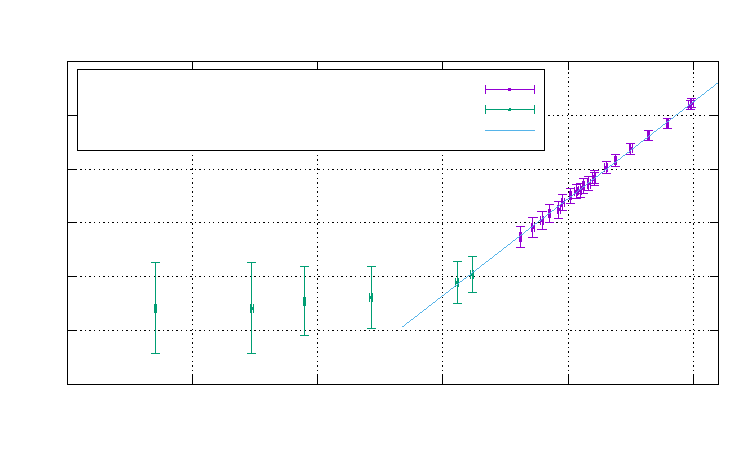
\includegraphics[width={360.00bp},height={216.00bp}]{305nm}}%
    \gplfronttext
  \end{picture}%
\endgroup

        \caption{a} \label{fig:photo_auswertung_305}
\end{figure*}
\begin{figure*}[h]
        \centering
        % GNUPLOT: LaTeX picture with Postscript
\begingroup
  \makeatletter
  \providecommand\color[2][]{%
    \GenericError{(gnuplot) \space\space\space\@spaces}{%
      Package color not loaded in conjunction with
      terminal option `colourtext'%
    }{See the gnuplot documentation for explanation.%
    }{Either use 'blacktext' in gnuplot or load the package
      color.sty in LaTeX.}%
    \renewcommand\color[2][]{}%
  }%
  \providecommand\includegraphics[2][]{%
    \GenericError{(gnuplot) \space\space\space\@spaces}{%
      Package graphicx or graphics not loaded%
    }{See the gnuplot documentation for explanation.%
    }{The gnuplot epslatex terminal needs graphicx.sty or graphics.sty.}%
    \renewcommand\includegraphics[2][]{}%
  }%
  \providecommand\rotatebox[2]{#2}%
  \@ifundefined{ifGPcolor}{%
    \newif\ifGPcolor
    \GPcolortrue
  }{}%
  \@ifundefined{ifGPblacktext}{%
    \newif\ifGPblacktext
    \GPblacktexttrue
  }{}%
  % define a \g@addto@macro without @ in the name:
  \let\gplgaddtomacro\g@addto@macro
  % define empty templates for all commands taking text:
  \gdef\gplbacktext{}%
  \gdef\gplfronttext{}%
  \makeatother
  \ifGPblacktext
    % no textcolor at all
    \def\colorrgb#1{}%
    \def\colorgray#1{}%
  \else
    % gray or color?
    \ifGPcolor
      \def\colorrgb#1{\color[rgb]{#1}}%
      \def\colorgray#1{\color[gray]{#1}}%
      \expandafter\def\csname LTw\endcsname{\color{white}}%
      \expandafter\def\csname LTb\endcsname{\color{black}}%
      \expandafter\def\csname LTa\endcsname{\color{black}}%
      \expandafter\def\csname LT0\endcsname{\color[rgb]{1,0,0}}%
      \expandafter\def\csname LT1\endcsname{\color[rgb]{0,1,0}}%
      \expandafter\def\csname LT2\endcsname{\color[rgb]{0,0,1}}%
      \expandafter\def\csname LT3\endcsname{\color[rgb]{1,0,1}}%
      \expandafter\def\csname LT4\endcsname{\color[rgb]{0,1,1}}%
      \expandafter\def\csname LT5\endcsname{\color[rgb]{1,1,0}}%
      \expandafter\def\csname LT6\endcsname{\color[rgb]{0,0,0}}%
      \expandafter\def\csname LT7\endcsname{\color[rgb]{1,0.3,0}}%
      \expandafter\def\csname LT8\endcsname{\color[rgb]{0.5,0.5,0.5}}%
    \else
      % gray
      \def\colorrgb#1{\color{black}}%
      \def\colorgray#1{\color[gray]{#1}}%
      \expandafter\def\csname LTw\endcsname{\color{white}}%
      \expandafter\def\csname LTb\endcsname{\color{black}}%
      \expandafter\def\csname LTa\endcsname{\color{black}}%
      \expandafter\def\csname LT0\endcsname{\color{black}}%
      \expandafter\def\csname LT1\endcsname{\color{black}}%
      \expandafter\def\csname LT2\endcsname{\color{black}}%
      \expandafter\def\csname LT3\endcsname{\color{black}}%
      \expandafter\def\csname LT4\endcsname{\color{black}}%
      \expandafter\def\csname LT5\endcsname{\color{black}}%
      \expandafter\def\csname LT6\endcsname{\color{black}}%
      \expandafter\def\csname LT7\endcsname{\color{black}}%
      \expandafter\def\csname LT8\endcsname{\color{black}}%
    \fi
  \fi
    \setlength{\unitlength}{0.0500bp}%
    \ifx\gptboxheight\undefined%
      \newlength{\gptboxheight}%
      \newlength{\gptboxwidth}%
      \newsavebox{\gptboxtext}%
    \fi%
    \setlength{\fboxrule}{0.5pt}%
    \setlength{\fboxsep}{1pt}%
    \definecolor{tbcol}{rgb}{1,1,1}%
\begin{picture}(7200.00,4320.00)%
    \gplgaddtomacro\gplbacktext{%
      \csname LTb\endcsname%%
      \put(536,619){\makebox(0,0)[r]{\strut{}$-4$}}%
      \csname LTb\endcsname%%
      \put(536,963){\makebox(0,0)[r]{\strut{}$-2$}}%
      \csname LTb\endcsname%%
      \put(536,1308){\makebox(0,0)[r]{\strut{}$0$}}%
      \csname LTb\endcsname%%
      \put(536,1652){\makebox(0,0)[r]{\strut{}$2$}}%
      \csname LTb\endcsname%%
      \put(536,1997){\makebox(0,0)[r]{\strut{}$4$}}%
      \csname LTb\endcsname%%
      \put(536,2341){\makebox(0,0)[r]{\strut{}$6$}}%
      \csname LTb\endcsname%%
      \put(536,2686){\makebox(0,0)[r]{\strut{}$8$}}%
      \csname LTb\endcsname%%
      \put(536,3030){\makebox(0,0)[r]{\strut{}$10$}}%
      \csname LTb\endcsname%%
      \put(536,3374){\makebox(0,0)[r]{\strut{}$12$}}%
      \csname LTb\endcsname%%
      \put(536,3719){\makebox(0,0)[r]{\strut{}$14$}}%
      \csname LTb\endcsname%%
      \put(634,425){\makebox(0,0){\strut{}$-2.5$}}%
      \csname LTb\endcsname%%
      \put(1836,425){\makebox(0,0){\strut{}$-2$}}%
      \csname LTb\endcsname%%
      \put(3038,425){\makebox(0,0){\strut{}$-1.5$}}%
      \csname LTb\endcsname%%
      \put(4241,425){\makebox(0,0){\strut{}$-1$}}%
      \csname LTb\endcsname%%
      \put(5443,425){\makebox(0,0){\strut{}$-0.5$}}%
      \csname LTb\endcsname%%
      \put(6645,425){\makebox(0,0){\strut{}$0$}}%
    }%
    \gplgaddtomacro\gplfronttext{%
      \csname LTb\endcsname%%
      \put(170,2169){\rotatebox{-270}{\makebox(0,0){\strut{}$\sqrt{I-I_0}$/mV}}}%
      \csname LTb\endcsname%%
      \put(3760,135){\makebox(0,0){\strut{}$U_G$/V}}%
      \csname LTb\endcsname%%
      \put(4745,3545){\makebox(0,0)[r]{\strut{}quadratische Datenpunkte}}%
      \csname LTb\endcsname%%
      \put(4745,3351){\makebox(0,0)[r]{\strut{}nicht quadratische Datenpunkte}}%
      \csname LTb\endcsname%%
      \put(4745,3158){\makebox(0,0)[r]{\strut{}$f(U_G)=\SI{7.649 +- 0.083}{}\cdot U_G + \SI{11.543 +- 0.040}{\milli V}$}}%
      \csname LTb\endcsname%%
      \put(3760,4009){\makebox(0,0){\strut{}$\lambda=\SI{365}{\nano m}$: $U_0=\SI{-1.509 +- 0.017}{V}$ und $\chi^2/\text{ddof}=\SI{0.389}{}$}}%
    }%
    \gplbacktext
    \put(0,0){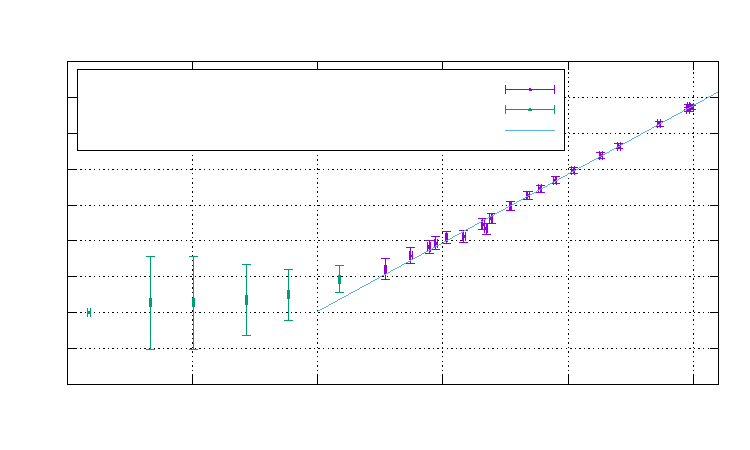
\includegraphics[width={360.00bp},height={216.00bp}]{365nm}}%
    \gplfronttext
  \end{picture}%
\endgroup

        \caption{a}
\end{figure*}
\begin{figure*}[h]
        \centering
        % GNUPLOT: LaTeX picture with Postscript
\begingroup
  \makeatletter
  \providecommand\color[2][]{%
    \GenericError{(gnuplot) \space\space\space\@spaces}{%
      Package color not loaded in conjunction with
      terminal option `colourtext'%
    }{See the gnuplot documentation for explanation.%
    }{Either use 'blacktext' in gnuplot or load the package
      color.sty in LaTeX.}%
    \renewcommand\color[2][]{}%
  }%
  \providecommand\includegraphics[2][]{%
    \GenericError{(gnuplot) \space\space\space\@spaces}{%
      Package graphicx or graphics not loaded%
    }{See the gnuplot documentation for explanation.%
    }{The gnuplot epslatex terminal needs graphicx.sty or graphics.sty.}%
    \renewcommand\includegraphics[2][]{}%
  }%
  \providecommand\rotatebox[2]{#2}%
  \@ifundefined{ifGPcolor}{%
    \newif\ifGPcolor
    \GPcolortrue
  }{}%
  \@ifundefined{ifGPblacktext}{%
    \newif\ifGPblacktext
    \GPblacktexttrue
  }{}%
  % define a \g@addto@macro without @ in the name:
  \let\gplgaddtomacro\g@addto@macro
  % define empty templates for all commands taking text:
  \gdef\gplbacktext{}%
  \gdef\gplfronttext{}%
  \makeatother
  \ifGPblacktext
    % no textcolor at all
    \def\colorrgb#1{}%
    \def\colorgray#1{}%
  \else
    % gray or color?
    \ifGPcolor
      \def\colorrgb#1{\color[rgb]{#1}}%
      \def\colorgray#1{\color[gray]{#1}}%
      \expandafter\def\csname LTw\endcsname{\color{white}}%
      \expandafter\def\csname LTb\endcsname{\color{black}}%
      \expandafter\def\csname LTa\endcsname{\color{black}}%
      \expandafter\def\csname LT0\endcsname{\color[rgb]{1,0,0}}%
      \expandafter\def\csname LT1\endcsname{\color[rgb]{0,1,0}}%
      \expandafter\def\csname LT2\endcsname{\color[rgb]{0,0,1}}%
      \expandafter\def\csname LT3\endcsname{\color[rgb]{1,0,1}}%
      \expandafter\def\csname LT4\endcsname{\color[rgb]{0,1,1}}%
      \expandafter\def\csname LT5\endcsname{\color[rgb]{1,1,0}}%
      \expandafter\def\csname LT6\endcsname{\color[rgb]{0,0,0}}%
      \expandafter\def\csname LT7\endcsname{\color[rgb]{1,0.3,0}}%
      \expandafter\def\csname LT8\endcsname{\color[rgb]{0.5,0.5,0.5}}%
    \else
      % gray
      \def\colorrgb#1{\color{black}}%
      \def\colorgray#1{\color[gray]{#1}}%
      \expandafter\def\csname LTw\endcsname{\color{white}}%
      \expandafter\def\csname LTb\endcsname{\color{black}}%
      \expandafter\def\csname LTa\endcsname{\color{black}}%
      \expandafter\def\csname LT0\endcsname{\color{black}}%
      \expandafter\def\csname LT1\endcsname{\color{black}}%
      \expandafter\def\csname LT2\endcsname{\color{black}}%
      \expandafter\def\csname LT3\endcsname{\color{black}}%
      \expandafter\def\csname LT4\endcsname{\color{black}}%
      \expandafter\def\csname LT5\endcsname{\color{black}}%
      \expandafter\def\csname LT6\endcsname{\color{black}}%
      \expandafter\def\csname LT7\endcsname{\color{black}}%
      \expandafter\def\csname LT8\endcsname{\color{black}}%
    \fi
  \fi
    \setlength{\unitlength}{0.0500bp}%
    \ifx\gptboxheight\undefined%
      \newlength{\gptboxheight}%
      \newlength{\gptboxwidth}%
      \newsavebox{\gptboxtext}%
    \fi%
    \setlength{\fboxrule}{0.5pt}%
    \setlength{\fboxsep}{1pt}%
    \definecolor{tbcol}{rgb}{1,1,1}%
\begin{picture}(7200.00,4320.00)%
    \gplgaddtomacro\gplbacktext{%
      \csname LTb\endcsname%%
      \put(536,766){\makebox(0,0)[r]{\strut{}$0$}}%
      \csname LTb\endcsname%%
      \put(536,1357){\makebox(0,0)[r]{\strut{}$2$}}%
      \csname LTb\endcsname%%
      \put(536,1947){\makebox(0,0)[r]{\strut{}$4$}}%
      \csname LTb\endcsname%%
      \put(536,2538){\makebox(0,0)[r]{\strut{}$6$}}%
      \csname LTb\endcsname%%
      \put(536,3128){\makebox(0,0)[r]{\strut{}$8$}}%
      \csname LTb\endcsname%%
      \put(536,3719){\makebox(0,0)[r]{\strut{}$10$}}%
      \csname LTb\endcsname%%
      \put(634,425){\makebox(0,0){\strut{}$-2.5$}}%
      \csname LTb\endcsname%%
      \put(1836,425){\makebox(0,0){\strut{}$-2$}}%
      \csname LTb\endcsname%%
      \put(3038,425){\makebox(0,0){\strut{}$-1.5$}}%
      \csname LTb\endcsname%%
      \put(4241,425){\makebox(0,0){\strut{}$-1$}}%
      \csname LTb\endcsname%%
      \put(5443,425){\makebox(0,0){\strut{}$-0.5$}}%
      \csname LTb\endcsname%%
      \put(6645,425){\makebox(0,0){\strut{}$0$}}%
    }%
    \gplgaddtomacro\gplfronttext{%
      \csname LTb\endcsname%%
      \put(4256,3448){\makebox(0,0)[r]{\strut{}quadratische Datenpunkte}}%
      \csname LTb\endcsname%%
      \put(4256,3255){\makebox(0,0)[r]{\strut{}nicht quadratische Datenpunkte}}%
      \csname LTb\endcsname%%
      \put(4256,3061){\makebox(0,0)[r]{\strut{}$f(U_G)=\SI{9.02 +- 0.10}{}\cdot U_G + \SI{8.575 +- 0.027}{\milli V}$}}%
      \csname LTb\endcsname%%
      \put(170,2169){\rotatebox{-270.00}{\makebox(0,0){\strut{}$\sqrt{I-I_0}$/mV}}}%
      \csname LTb\endcsname%%
      \put(3760,135){\makebox(0,0){\strut{}$U_G$/V}}%
      \csname LTb\endcsname%%
      \put(3760,4009){\makebox(0,0){\strut{}$\lambda=\SI{436}{\nano m}$: $U_0=\SI{-0.951 +- 0.000}{V}$ und $\chi^2/\text{ddof}=\SI{0.103}{}$}}%
    }%
    \gplbacktext
    \put(0,0){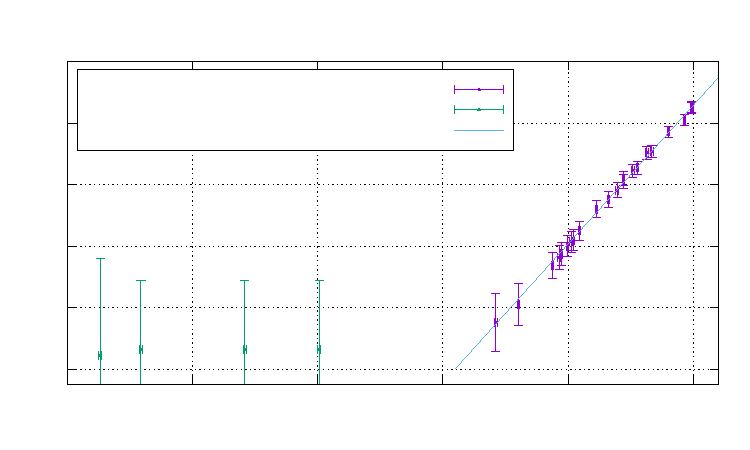
\includegraphics[width={360.00bp},height={216.00bp}]{436nm}}%
    \gplfronttext
  \end{picture}%
\endgroup

        \caption{a}
\end{figure*}
\begin{figure*}[]
        \centering
        % GNUPLOT: LaTeX picture with Postscript
\begingroup
  \makeatletter
  \providecommand\color[2][]{%
    \GenericError{(gnuplot) \space\space\space\@spaces}{%
      Package color not loaded in conjunction with
      terminal option `colourtext'%
    }{See the gnuplot documentation for explanation.%
    }{Either use 'blacktext' in gnuplot or load the package
      color.sty in LaTeX.}%
    \renewcommand\color[2][]{}%
  }%
  \providecommand\includegraphics[2][]{%
    \GenericError{(gnuplot) \space\space\space\@spaces}{%
      Package graphicx or graphics not loaded%
    }{See the gnuplot documentation for explanation.%
    }{The gnuplot epslatex terminal needs graphicx.sty or graphics.sty.}%
    \renewcommand\includegraphics[2][]{}%
  }%
  \providecommand\rotatebox[2]{#2}%
  \@ifundefined{ifGPcolor}{%
    \newif\ifGPcolor
    \GPcolortrue
  }{}%
  \@ifundefined{ifGPblacktext}{%
    \newif\ifGPblacktext
    \GPblacktexttrue
  }{}%
  % define a \g@addto@macro without @ in the name:
  \let\gplgaddtomacro\g@addto@macro
  % define empty templates for all commands taking text:
  \gdef\gplbacktext{}%
  \gdef\gplfronttext{}%
  \makeatother
  \ifGPblacktext
    % no textcolor at all
    \def\colorrgb#1{}%
    \def\colorgray#1{}%
  \else
    % gray or color?
    \ifGPcolor
      \def\colorrgb#1{\color[rgb]{#1}}%
      \def\colorgray#1{\color[gray]{#1}}%
      \expandafter\def\csname LTw\endcsname{\color{white}}%
      \expandafter\def\csname LTb\endcsname{\color{black}}%
      \expandafter\def\csname LTa\endcsname{\color{black}}%
      \expandafter\def\csname LT0\endcsname{\color[rgb]{1,0,0}}%
      \expandafter\def\csname LT1\endcsname{\color[rgb]{0,1,0}}%
      \expandafter\def\csname LT2\endcsname{\color[rgb]{0,0,1}}%
      \expandafter\def\csname LT3\endcsname{\color[rgb]{1,0,1}}%
      \expandafter\def\csname LT4\endcsname{\color[rgb]{0,1,1}}%
      \expandafter\def\csname LT5\endcsname{\color[rgb]{1,1,0}}%
      \expandafter\def\csname LT6\endcsname{\color[rgb]{0,0,0}}%
      \expandafter\def\csname LT7\endcsname{\color[rgb]{1,0.3,0}}%
      \expandafter\def\csname LT8\endcsname{\color[rgb]{0.5,0.5,0.5}}%
    \else
      % gray
      \def\colorrgb#1{\color{black}}%
      \def\colorgray#1{\color[gray]{#1}}%
      \expandafter\def\csname LTw\endcsname{\color{white}}%
      \expandafter\def\csname LTb\endcsname{\color{black}}%
      \expandafter\def\csname LTa\endcsname{\color{black}}%
      \expandafter\def\csname LT0\endcsname{\color{black}}%
      \expandafter\def\csname LT1\endcsname{\color{black}}%
      \expandafter\def\csname LT2\endcsname{\color{black}}%
      \expandafter\def\csname LT3\endcsname{\color{black}}%
      \expandafter\def\csname LT4\endcsname{\color{black}}%
      \expandafter\def\csname LT5\endcsname{\color{black}}%
      \expandafter\def\csname LT6\endcsname{\color{black}}%
      \expandafter\def\csname LT7\endcsname{\color{black}}%
      \expandafter\def\csname LT8\endcsname{\color{black}}%
    \fi
  \fi
    \setlength{\unitlength}{0.0500bp}%
    \ifx\gptboxheight\undefined%
      \newlength{\gptboxheight}%
      \newlength{\gptboxwidth}%
      \newsavebox{\gptboxtext}%
    \fi%
    \setlength{\fboxrule}{0.5pt}%
    \setlength{\fboxsep}{1pt}%
    \definecolor{tbcol}{rgb}{1,1,1}%
\begin{picture}(7200.00,4320.00)%
    \gplgaddtomacro\gplbacktext{%
      \csname LTb\endcsname%%
      \put(536,766){\makebox(0,0)[r]{\strut{}$0$}}%
      \csname LTb\endcsname%%
      \put(536,1357){\makebox(0,0)[r]{\strut{}$2$}}%
      \csname LTb\endcsname%%
      \put(536,1947){\makebox(0,0)[r]{\strut{}$4$}}%
      \csname LTb\endcsname%%
      \put(536,2538){\makebox(0,0)[r]{\strut{}$6$}}%
      \csname LTb\endcsname%%
      \put(536,3128){\makebox(0,0)[r]{\strut{}$8$}}%
      \csname LTb\endcsname%%
      \put(536,3719){\makebox(0,0)[r]{\strut{}$10$}}%
      \csname LTb\endcsname%%
      \put(634,425){\makebox(0,0){\strut{}$-2.5$}}%
      \csname LTb\endcsname%%
      \put(1836,425){\makebox(0,0){\strut{}$-2$}}%
      \csname LTb\endcsname%%
      \put(3038,425){\makebox(0,0){\strut{}$-1.5$}}%
      \csname LTb\endcsname%%
      \put(4241,425){\makebox(0,0){\strut{}$-1$}}%
      \csname LTb\endcsname%%
      \put(5443,425){\makebox(0,0){\strut{}$-0.5$}}%
      \csname LTb\endcsname%%
      \put(6645,425){\makebox(0,0){\strut{}$0$}}%
    }%
    \gplgaddtomacro\gplfronttext{%
      \csname LTb\endcsname%%
      \put(4354,3545){\makebox(0,0)[r]{\strut{}quadratische Datenpunkte}}%
      \csname LTb\endcsname%%
      \put(4354,3351){\makebox(0,0)[r]{\strut{}nicht quadratische Datenpunkte}}%
      \csname LTb\endcsname%%
      \put(4354,3158){\makebox(0,0)[r]{\strut{}$f(U_G)=\SI{32.88 +- 0.70}{}\cdot U_G + \SI{8.599 +- 0.042}{\milli V}$}}%
      \csname LTb\endcsname%%
      \put(170,2169){\rotatebox{-270.00}{\makebox(0,0){\strut{}$\sqrt{I-I_0}$/mV}}}%
      \csname LTb\endcsname%%
      \put(3760,135){\makebox(0,0){\strut{}$U_G$/V}}%
      \csname LTb\endcsname%%
      \put(3760,4009){\makebox(0,0){\strut{}$\lambda=\SI{546}{\nano m}$: $U_0=\SI{-0.2615 +- 0.0057}{V}$ und $\chi^2/\text{ddof}=\SI{0.195}{}$}}%
    }%
    \gplbacktext
    \put(0,0){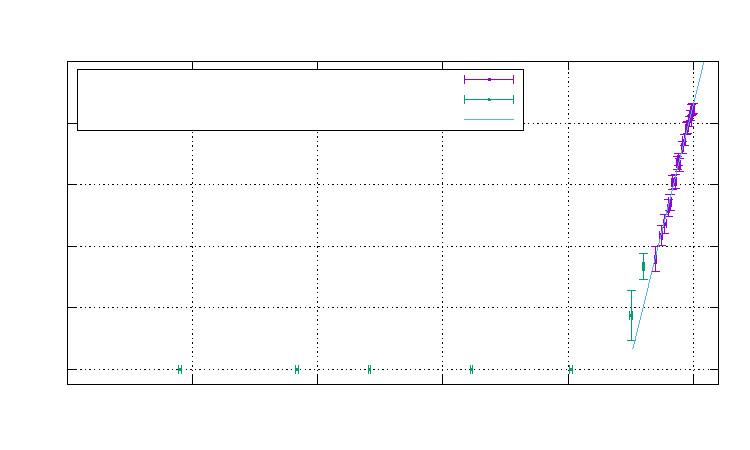
\includegraphics[width={360.00bp},height={216.00bp}]{546nm}}%
    \gplfronttext
  \end{picture}%
\endgroup

        \caption{a}
\end{figure*}
\begin{figure*}[]
        \centering
        % GNUPLOT: LaTeX picture with Postscript
\begingroup
  \makeatletter
  \providecommand\color[2][]{%
    \GenericError{(gnuplot) \space\space\space\@spaces}{%
      Package color not loaded in conjunction with
      terminal option `colourtext'%
    }{See the gnuplot documentation for explanation.%
    }{Either use 'blacktext' in gnuplot or load the package
      color.sty in LaTeX.}%
    \renewcommand\color[2][]{}%
  }%
  \providecommand\includegraphics[2][]{%
    \GenericError{(gnuplot) \space\space\space\@spaces}{%
      Package graphicx or graphics not loaded%
    }{See the gnuplot documentation for explanation.%
    }{The gnuplot epslatex terminal needs graphicx.sty or graphics.sty.}%
    \renewcommand\includegraphics[2][]{}%
  }%
  \providecommand\rotatebox[2]{#2}%
  \@ifundefined{ifGPcolor}{%
    \newif\ifGPcolor
    \GPcolortrue
  }{}%
  \@ifundefined{ifGPblacktext}{%
    \newif\ifGPblacktext
    \GPblacktexttrue
  }{}%
  % define a \g@addto@macro without @ in the name:
  \let\gplgaddtomacro\g@addto@macro
  % define empty templates for all commands taking text:
  \gdef\gplbacktext{}%
  \gdef\gplfronttext{}%
  \makeatother
  \ifGPblacktext
    % no textcolor at all
    \def\colorrgb#1{}%
    \def\colorgray#1{}%
  \else
    % gray or color?
    \ifGPcolor
      \def\colorrgb#1{\color[rgb]{#1}}%
      \def\colorgray#1{\color[gray]{#1}}%
      \expandafter\def\csname LTw\endcsname{\color{white}}%
      \expandafter\def\csname LTb\endcsname{\color{black}}%
      \expandafter\def\csname LTa\endcsname{\color{black}}%
      \expandafter\def\csname LT0\endcsname{\color[rgb]{1,0,0}}%
      \expandafter\def\csname LT1\endcsname{\color[rgb]{0,1,0}}%
      \expandafter\def\csname LT2\endcsname{\color[rgb]{0,0,1}}%
      \expandafter\def\csname LT3\endcsname{\color[rgb]{1,0,1}}%
      \expandafter\def\csname LT4\endcsname{\color[rgb]{0,1,1}}%
      \expandafter\def\csname LT5\endcsname{\color[rgb]{1,1,0}}%
      \expandafter\def\csname LT6\endcsname{\color[rgb]{0,0,0}}%
      \expandafter\def\csname LT7\endcsname{\color[rgb]{1,0.3,0}}%
      \expandafter\def\csname LT8\endcsname{\color[rgb]{0.5,0.5,0.5}}%
    \else
      % gray
      \def\colorrgb#1{\color{black}}%
      \def\colorgray#1{\color[gray]{#1}}%
      \expandafter\def\csname LTw\endcsname{\color{white}}%
      \expandafter\def\csname LTb\endcsname{\color{black}}%
      \expandafter\def\csname LTa\endcsname{\color{black}}%
      \expandafter\def\csname LT0\endcsname{\color{black}}%
      \expandafter\def\csname LT1\endcsname{\color{black}}%
      \expandafter\def\csname LT2\endcsname{\color{black}}%
      \expandafter\def\csname LT3\endcsname{\color{black}}%
      \expandafter\def\csname LT4\endcsname{\color{black}}%
      \expandafter\def\csname LT5\endcsname{\color{black}}%
      \expandafter\def\csname LT6\endcsname{\color{black}}%
      \expandafter\def\csname LT7\endcsname{\color{black}}%
      \expandafter\def\csname LT8\endcsname{\color{black}}%
    \fi
  \fi
    \setlength{\unitlength}{0.0500bp}%
    \ifx\gptboxheight\undefined%
      \newlength{\gptboxheight}%
      \newlength{\gptboxwidth}%
      \newsavebox{\gptboxtext}%
    \fi%
    \setlength{\fboxrule}{0.5pt}%
    \setlength{\fboxsep}{1pt}%
    \definecolor{tbcol}{rgb}{1,1,1}%
\begin{picture}(7200.00,4320.00)%
    \gplgaddtomacro\gplbacktext{%
      \csname LTb\endcsname%%
      \put(536,766){\makebox(0,0)[r]{\strut{}$0$}}%
      \csname LTb\endcsname%%
      \put(536,1357){\makebox(0,0)[r]{\strut{}$2$}}%
      \csname LTb\endcsname%%
      \put(536,1947){\makebox(0,0)[r]{\strut{}$4$}}%
      \csname LTb\endcsname%%
      \put(536,2538){\makebox(0,0)[r]{\strut{}$6$}}%
      \csname LTb\endcsname%%
      \put(536,3128){\makebox(0,0)[r]{\strut{}$8$}}%
      \csname LTb\endcsname%%
      \put(536,3719){\makebox(0,0)[r]{\strut{}$10$}}%
      \csname LTb\endcsname%%
      \put(634,425){\makebox(0,0){\strut{}$-2.5$}}%
      \csname LTb\endcsname%%
      \put(1836,425){\makebox(0,0){\strut{}$-2$}}%
      \csname LTb\endcsname%%
      \put(3038,425){\makebox(0,0){\strut{}$-1.5$}}%
      \csname LTb\endcsname%%
      \put(4241,425){\makebox(0,0){\strut{}$-1$}}%
      \csname LTb\endcsname%%
      \put(5443,425){\makebox(0,0){\strut{}$-0.5$}}%
      \csname LTb\endcsname%%
      \put(6645,425){\makebox(0,0){\strut{}$0$}}%
    }%
    \gplgaddtomacro\gplfronttext{%
      \csname LTb\endcsname%%
      \put(4354,3448){\makebox(0,0)[r]{\strut{}quadratische Datenpunkte}}%
      \csname LTb\endcsname%%
      \put(4354,3255){\makebox(0,0)[r]{\strut{}nicht quadratische Datenpunkte}}%
      \csname LTb\endcsname%%
      \put(4354,3061){\makebox(0,0)[r]{\strut{}$f(U_G)=\SI{20.88 +- 0.77}{}\cdot U_G + \SI{8.108 +- 0.075}{\milli V}$}}%
      \csname LTb\endcsname%%
      \put(170,2169){\rotatebox{-270.00}{\makebox(0,0){\strut{}$\sqrt{I-I_0}$/mV}}}%
      \csname LTb\endcsname%%
      \put(3760,135){\makebox(0,0){\strut{}$U_G$/V}}%
      \csname LTb\endcsname%%
      \put(3760,4009){\makebox(0,0){\strut{}$\lambda=\SI{578}{\nano m}$: $U_0=\SI{-0.388 +- 0.000}{V}$ und $\chi^2/\text{ddof}=\SI{0.850}{}$}}%
    }%
    \gplbacktext
    \put(0,0){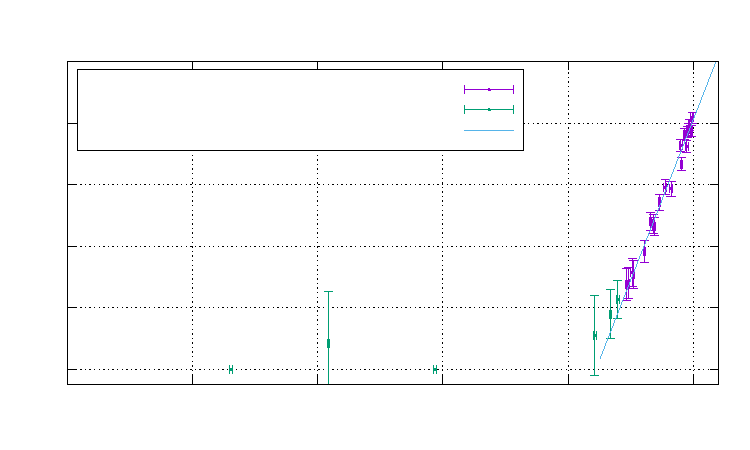
\includegraphics[width={360.00bp},height={216.00bp}]{578nm}}%
    \gplfronttext
  \end{picture}%
\endgroup

        \caption{a} \label{fig:photo_auswertung_578}
\end{figure*}

\clearpage
\bibliography{refs}

\end{document}
